In this section we will explain how our group organised and how we managed our work.

At the start of the project during our initial planning session, the group committed to a custom flavour of the popular `Kanban' methodology where we dropped parts that did not work for our team. Our philosophy in adapting Kanban to our needs was that `our process should work for us – we should not work for our process'.

As our project involved contributing to an existing codebase, we also decided to spend the first week familiarising ourselves with the codebase. This was important for the whole group to contribute effectively, especially as most had no prior experience with the Swift programming language.

We spent the first week updating the open source project to run on the latest version of Swift as it had not been worked on for several months at that point. We also added a code linting tool called `SwiftLint'\footnote{\url{https://github.com/realm/SwiftLint}} to the build pipeline in order to ensure that all code is formatted consistently.

\section{Planning}

Every week we had a meeting on Mondays at 16:00, where we all came together and reflected on the work of the past week. Many of these meetings had interesting and heated discussions about matters of design and which direction to take the project in. Additionally the Monday meeting served as a meeting where we were able to plan the next week of work, such as features we would like to work on as well as tickets that needed to be completed for a feature to be complete.

On Wednesdays our group would meet with our supervisor to discuss our progress and what features we felt we should work on. From this process many of the features that we worked on which were not originally planned emerged, such as the work on unit testing. We would also use this as an opportunity to demonstrate our work from the two weeks prior and get the milestone assessment sheets signed in weeks where they were due.

Every day we had a virtual standup meetings on our \#standups Slack channel. Group members were notified through a daily reminder that was set up on this channel, and asked to write a small message about what they were working on and whether they needed any help from the rest of the group. No message was required from individuals who had not done any work since the last meeting. Initially we had these meetings only once during the day at 11:00, but at the start of Checkpoint 3 we decided to hold an additional meeting at 19:00. By holding two standup meetings we could coordinate more effectively with the schedules of all group members, as some member had lectures in the morning and therefore could not work on the project until the afternoon and vice versa. We noticed significantly higher participation in these meetings by having two each day rather than just one, as group members who did not work in the mornings would often miss the notification from the morning meeting.

Halfway through the project, at the end of the second checkpoint, we met to look at our progress and think about how we can change the process to make a success of the latter two checkpoints of the project. We used a website called `Retrium' which allowed us to anonymously contribute thoughts as a set of virtual notes organised into several columns labelled `start', `stop', and `continue' (see figure \ref{retrium}). It was in this meeting that we identified that we wanted to have multiple standups a day and that we should work harder to not get sidetracked. One issue throughout the project was that implementing some features required the investment of a significant amount of time to build the necessary foundations.

\begin{figure}[htpb]
\centering
\makebox[\textwidth]{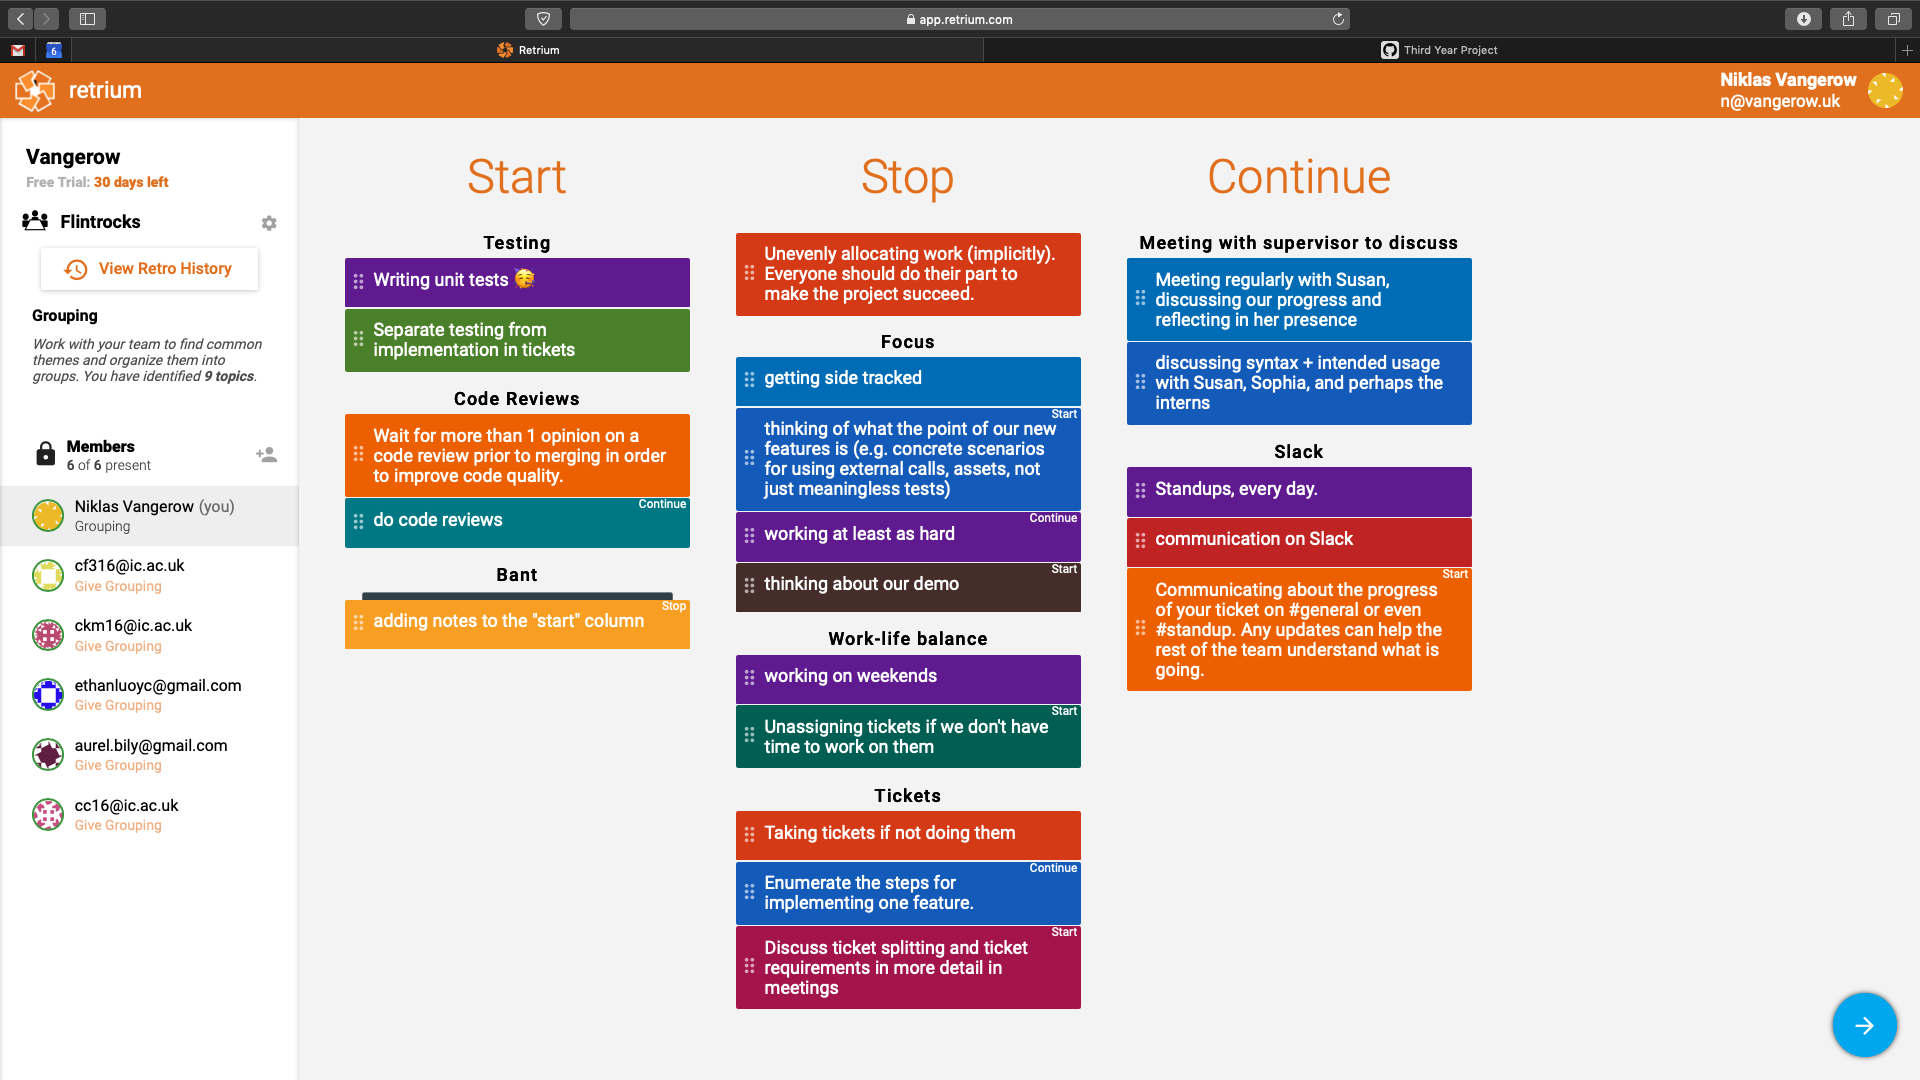
\includegraphics[width=\textwidth]{figures/Retrospective/r1.png}}
\caption{Our Retrium board showing all suggestions made by the team.}
\label{retrium}
\end{figure}

\section{Organisation}

\subsection{Process}

We chose Kanban as we wanted the flexibility of taking up new work as it happened while at the same time being aware of the work that is still pending. Our version of Kanban removed the WIP limit and instead enforced a softer limit that any one person could only be working on one ticket at any time. This kept the number of concurrent tickets low, but as the WIP limit was 6 there was less overlap and thus less need for individuals to pair. 

We chose not to adopt a Scrum methodology as we deemed it to be too inflexible for our individual schedules due to vastly disparate course choices. Scrum would have forced long meetings committing to specific pieces of work ahead of time when the scope of our project was constantly changing.

\subsection{Project Board}

To give every team member the ability to see the progress of the project at a glance and indicate the progress of their own work, we opted to use a `ticket' system, which is very common in Agile workflows. Each task (or ticket) was first created as a vague `research' task that required research and scoping. A completed research task would result in the creation of many new tickets that could be worked on by developers containing sufficient detail in order to achieve the task at hand as well as a notion of order and dependence between these tickets. The group member who completed the relevant research ticket also became the owner of the work contained and was encouraged to take ownership and be ready to provide clarification when something was unclear.

Our project board served to organise these tasks into logical categories while showing a clear progression in the status of the ticket. The original categories that we had stemmed from GitHub's Kanban template and were the following:

\begin{figure}[H]
\centering
\begin{tikzpicture}[%
	main node/.style={
		rectangle,
		fill=gray!20,
		draw,
		minimum width=2.65cm,
		minimum height=1cm,
		inner sep=0pt,
		anchor=mid,
		text height=1.5ex,
		text depth=.25ex,
	}
]
	\node[main node] (1) {To do};
	\node[main node] (2) [right = 1cm of 1] {In progress};
	\node[main node] (3) [right = 1cm of 2] {Needs review};
	\node[main node] (4) [right = 1cm of 3] {Done};
	\path[draw,thick,->]
	(1) edge node {} (2)
	(2) edge node {} (3)
	(3) edge node {} (4);
\end{tikzpicture}
%\caption{}
%\label{}
\end{figure}

Following our first consultation meeting with Dr Robert Chatley we decided to make fundamental changes to our board which would persist for the remainder of the project. First, we changed the categories to this progression:

\begin{figure}[H]
\centering
\begin{tikzpicture}[%
	main node/.style={
		rectangle,
		fill=gray!20,
		draw,
		minimum width=2.45cm,
		minimum height=1.3cm,
		inner sep=0pt,
		%text height=1.5ex,
		text width=2.45cm,
		%text depth=.25ex,
		align=center
	}
]
	\node[main node] (1) {Needs review};
	\node[main node] (2) [right = .5cm of 1] {Needs development};
	\node[main node] (3) [right = .5cm of 2] {Needs analysis};
	\node[main node] (4) [right = .5cm of 3] {To do};
	\node[main node] (5) [right = .5cm of 4] {Done};
	\path[draw,thick,->]
	(4) edge node {} (3)
	(3) edge node {} (2)
	(2) edge node {} (1);
	\path[draw,thick,->]
	(1.south) edge[bend right=10] node {} (5.south);
\end{tikzpicture}
%\caption{}
%\label{}
\end{figure}

and inverted the order to emphasise that it is preferable to complete 80\% of tickets 100\% of the way rather than 100\% of the tickets only 80\% of the way. On this board work moved from the right to the left. It was not a lot of work for the group to get used to this new board as most of the tickets would move automatically thanks to GitHub's automation feature. 

With work moving from the right to the left, whenever the board is first opened the tickets that need to be code-reviewed show up first. We decided that the order of work for everyone should be to 1. review all tickets in the `needs review' column, 2. complete all tickets in the `needs development' column, etc. This way we ensured that all completed tickets were reviewed by at least one person and that the review happened as soon as possible. Figure \ref{board} shows the reconfigured board.

\begin{figure}[htbp]
\centering
\makebox[\textwidth]{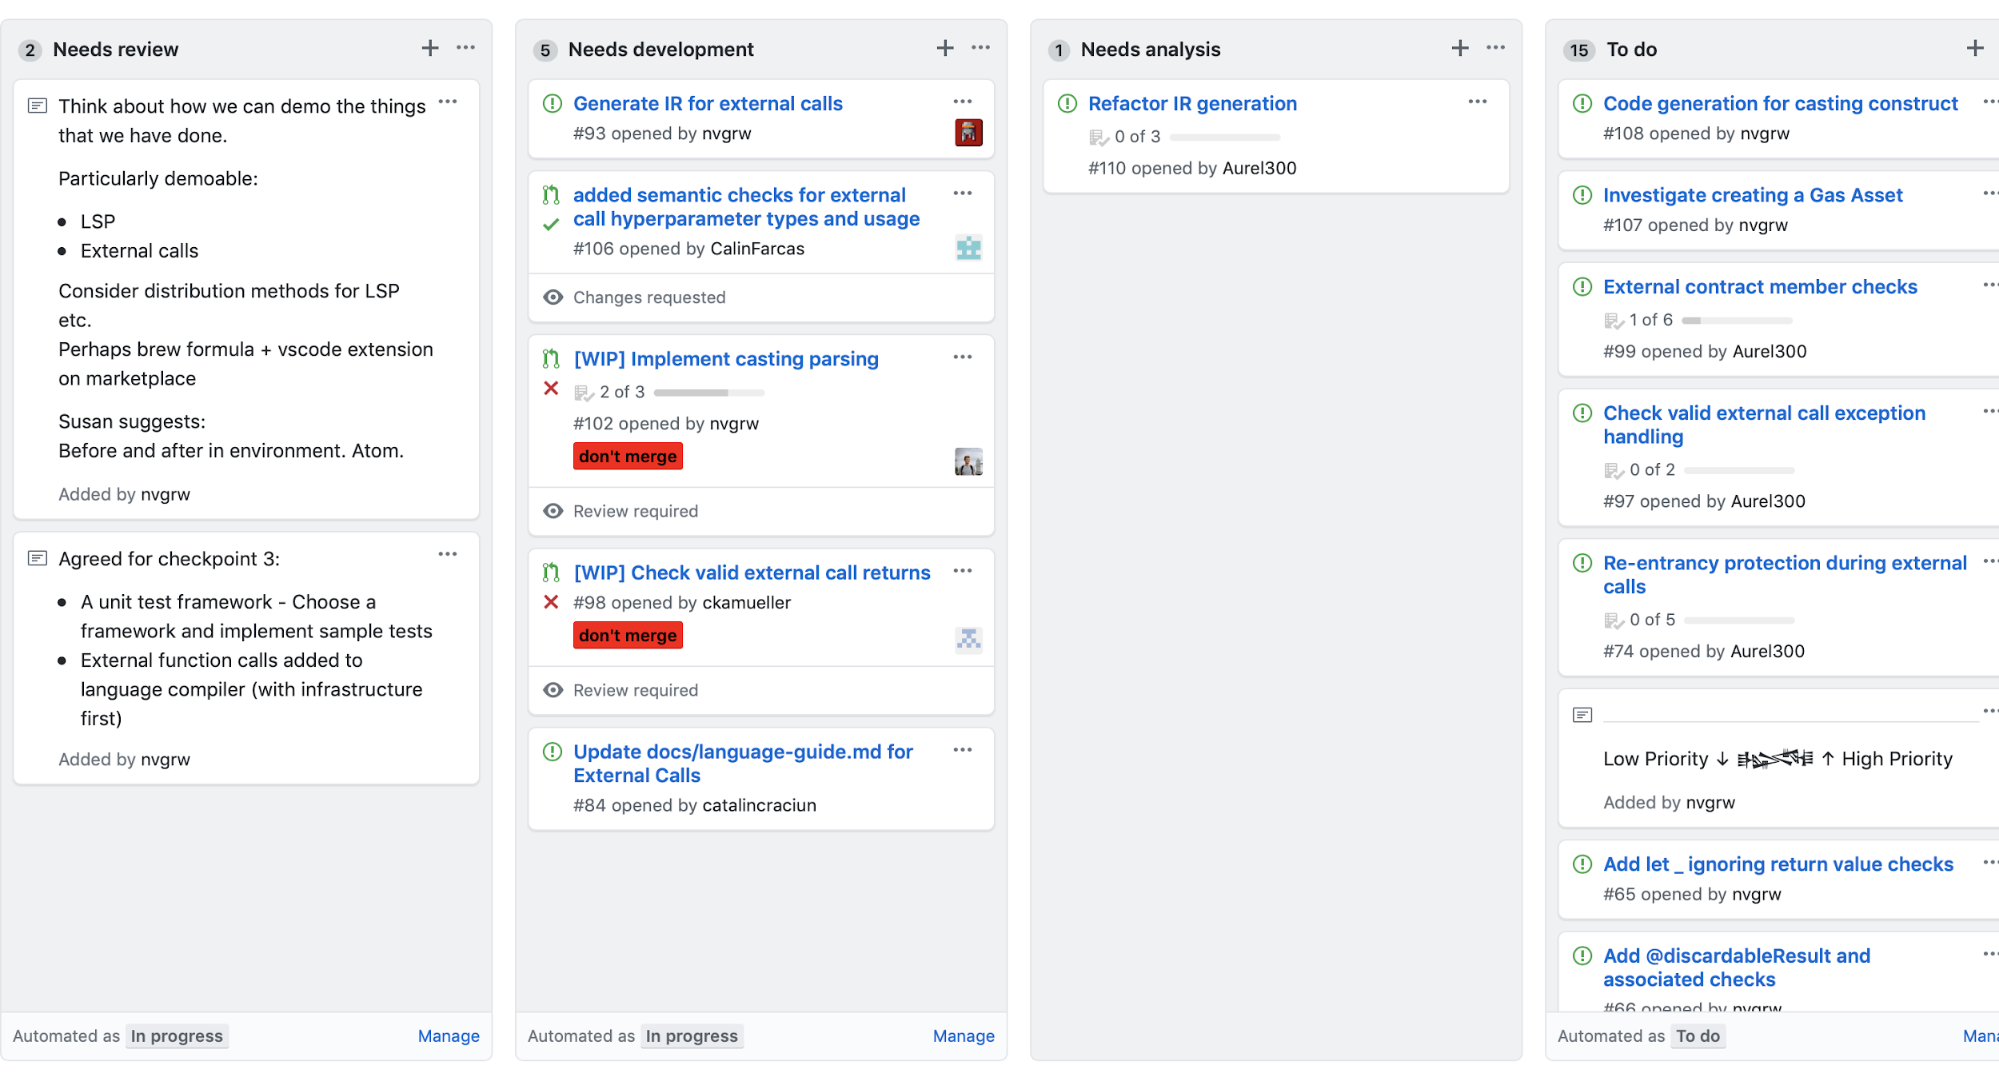
\includegraphics[width=\textwidth]{figures/board-cp3.png}}
\caption{The project board at the start of the third iteration.}
\label{board}
\end{figure}

In addition to the board, we used GitHub's milestones feature to track the progress on some of our `sub-projects' such as external calls, unit testing, and asset traits. Figure \ref{milestones} shows that milestones provide a handy progression bar that reflects the tickets' current status on the board.

\begin{figure}[htbp]
\centering
\makebox[\textwidth]{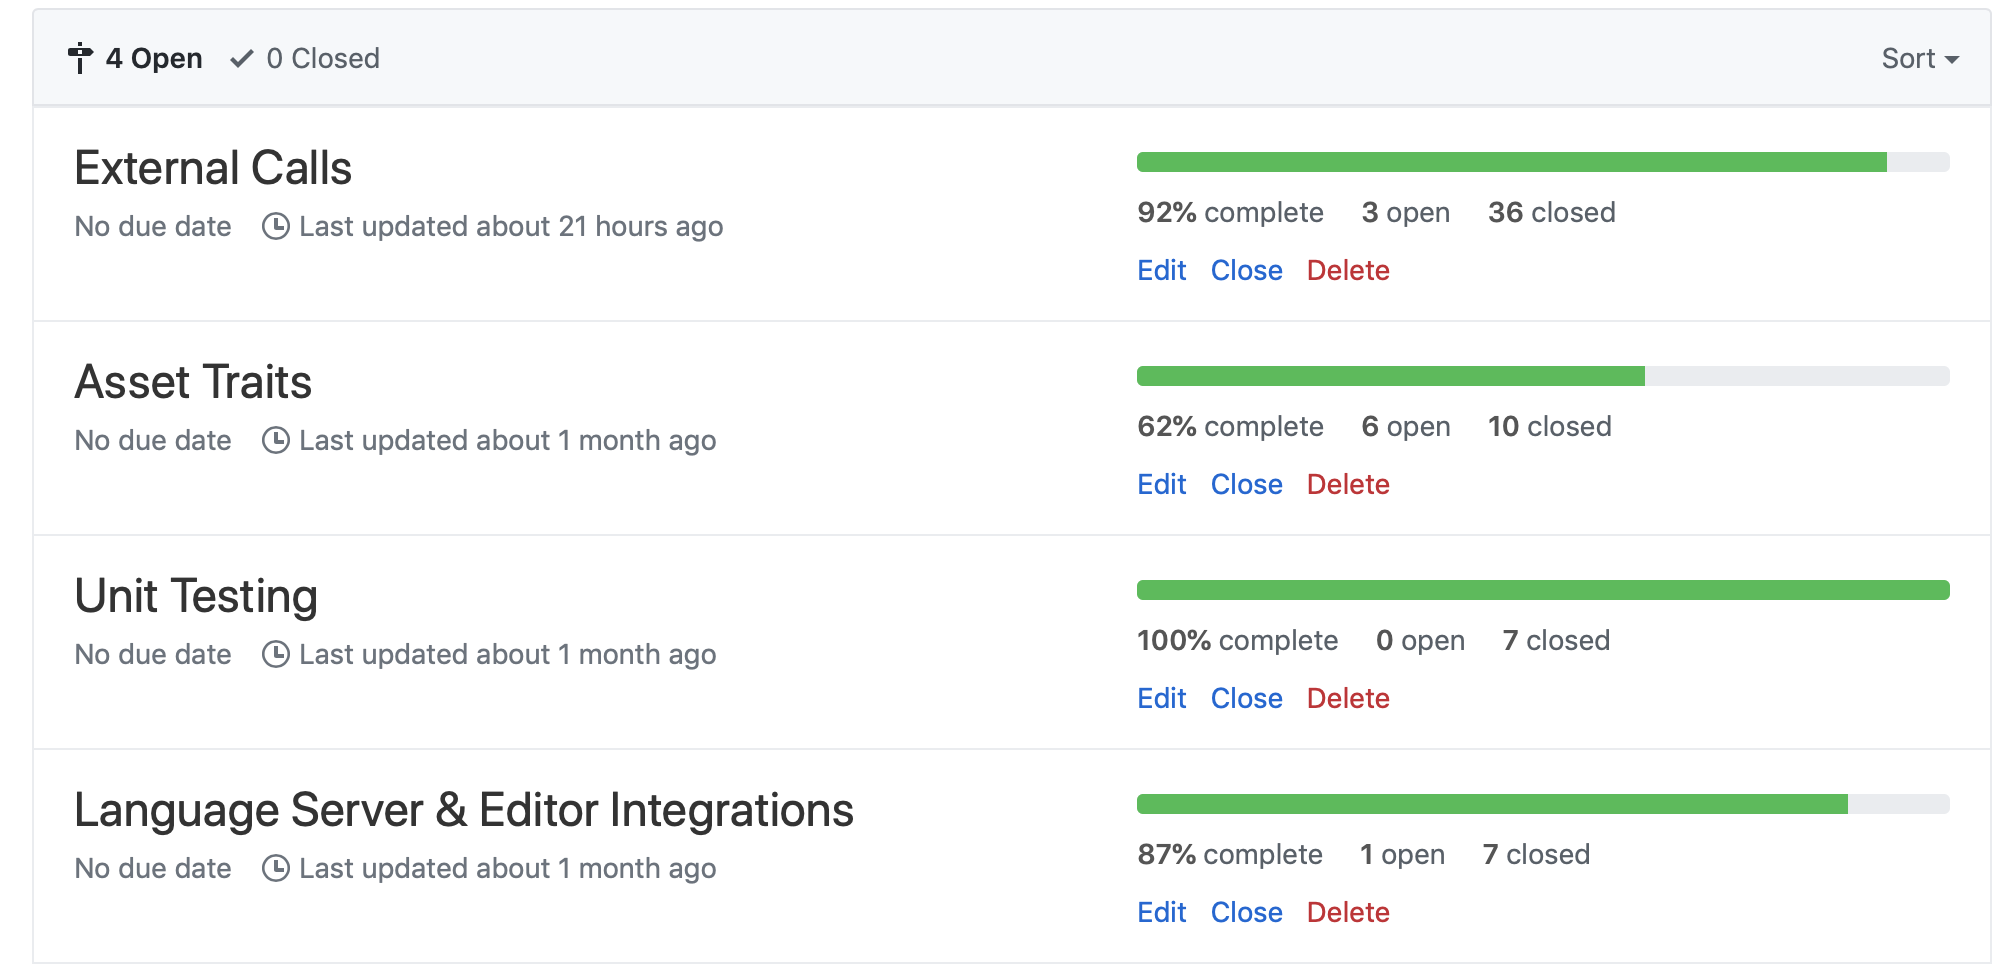
\includegraphics[width=\textwidth]{figures/milestones.png}}
\caption{Milestones on our GitHub repository.}
\label{milestones}
\end{figure}

\subsection{Review Process}

Each ticket corresponded to a `feature' branch on our GitHub repository. We made an effort to enforce a strict review process with a continuous integration pipeline which ensured that every patch worked both before and after merging, as well as to ensure that the code being committed complied with our codebase style rules. To enforce style, we used a tool called swiftlint which would make our build fail if there was an extraneous space or other formatting issue. Once a ticket was nearing completion, a corresponding pull request was created which referenced the issue number of the ticket. This meant that the ticket would automatically be closed when the pull request was closed due to merging or due to being superseded by another ticket or pull request.

Generally our group was very flexible about whose approval was required for any particular feature to be merged. Originally we did not want roles but it very quickly became apparent that some hierarchy was required to make progress. As a result, most code reviews would be reviewed by the `project master' as well as a number of group members before merging (see figure \ref{pr}). Occasionally when it was necessary, group members also had the freedom to bypass the review process from the project master and approve code changes themselves. This flexibility was a tradeoff between moving fast and ensuring that the code quality remains high.

\begin{figure}[htbp]
\centering
\makebox[\textwidth]{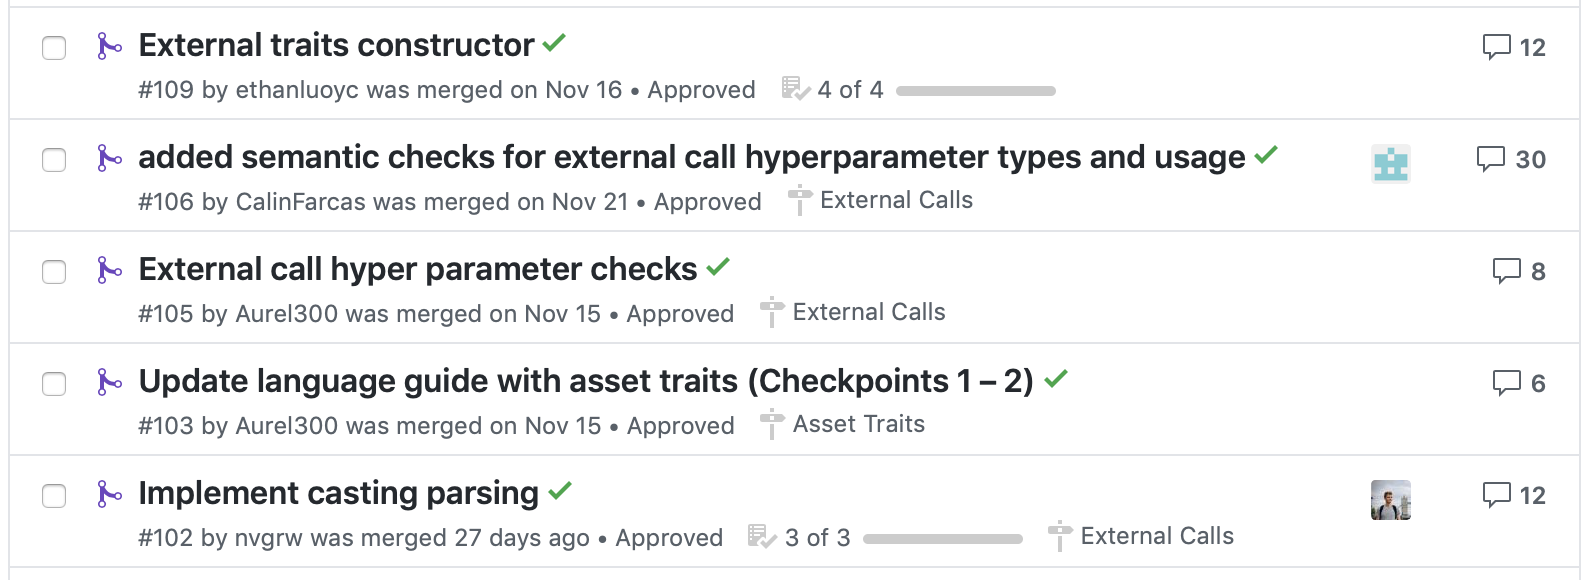
\includegraphics[width=\textwidth]{figures/pr-discussion.png}}
\caption{Some merged pull requests. Note the number of comments on the right-hand side.}
\label{pr}
\end{figure}

We merged features only through squashing and merging in to the mainline master branch. This branch was protected from pushes and could only be modified through the GitHub user interface on pull requests to enforce the review process. A squash, in git parlance, refers to the act of taking a set of commits and combining them into a single commit. Squashing commits is a very common practice in large companies utilising source control and particularly in those that utilise a monolithic repository (monorepo) for dependency management. Additionally it meant that group members did not feel the need to measure themselves by their number of commits, as the only measurable metric was the contribution of features, which were far more important for the project. Enforcing the squashing of commits kept the history of the repository cleaner, made it easier to revert changes should they need to be reverted, as well as allowing group members to make many commits and experiment within their own branch in order to deliver a feature that was the best that it could be.

\subsection{Communication}

Our primary means of communication was Slack. Although the team was slow to adapt to Slack initially, preferring a Messenger chat instead, we soon warmed up to it and made full use of its features. In our Slack group we had some key messaging channels: \#general was for communications that concerned the project in general, or for anyone needing help or clarification on something; \#ask-for-code-review had a GitHub bot that would automatically ping all group members as soon as there was any activity on the repository (merges into master, opening and closing of pull requests, new issues created, etc) in order to keep all members in the loop; \#standups had a daily message at 11:00 and 19:00 to remind everyone to write a brief message about what they were working on.

\section{Task Allocation and Roles}

We had originally planned to split our group into two sub-groups where each sub-group works on one aspect of the project, specifically the integration with the language server and the language extensions. We ended up primarily focusing on the language extensions and therefore this clear `split' only persisted for about a week into the project. More often than not, we had a team member take charge of a particular task and delegate as needed.

We tried to encourage pairing as much as possible in order to meet our prescribed bi-weekly deadlines for the milestone assessments. If a team member struggled to complete their feature by a deadline they were constantly encouraged to get help from another team member to get their feature completed or even to hand it off to another group member.

Unlike commonly done in other Agile workflows, we chose to not allocate tasks to any individual at the task creation stage. This saved us significant time in meetings and allowed us to focus on making tickets descriptive and ensuring that everyone was on track. Instead, the group worked on the basis that everyone would put in roughly the same amount of work and could therefore pick up a ticket that was not already being worked on from the backlog once there were no more patches to review. New tickets were always spawned from research tickets and prioritised at the Monday meetings to conform with our milestone commitments to our supervisor.

Despite our original idea of not having roles, at some point the group needed leadership so a leader (project master) was elected:

\begin{center}
	\begin{tabular}{ll}
		Member & Role\\\hline
		Aurel Bílý & Developer\\
		Catalin Craciun & Developer\\
		Calin Farcas & Developer\\
		Yicheng Luo & Developer\\
		Constantin Mueller & Developer\\
		Niklas Vangerow & Developer and Project Master
	\end{tabular}
\end{center}

Developers contributed to the project as described above, by creating feature branches, pull requests, and merging these features. The project master had the additional responsibility of organising and leading group meetings, ensuring that checkpoint documents were completed on time, as well as being the ultimate authority on code that enters the master branch. Our group was small and it was impractical to only have 5 developers, so the project master role also involved normal feature development.
